% !TEX TS-program = XeLaTeX
% use the following command:
% all document files must be coded in UTF-8
\documentclass[english]{textolivre}
% build HTML with: make4ht -e build.lua -c textolivre.cfg -x -u article "fn-in,svg,pic-align"

\journalname{Texto Livre}
\thevolume{16}
%\thenumber{1} % old template
\theyear{2023}
\receiveddate{\DTMdisplaydate{2023}{5}{4}{-1}} % YYYY MM DD
\accepteddate{\DTMdisplaydate{2023}{7}{31}{-1}}
\publisheddate{\today}
\corrauthor{Laura Ribeiro Araújo}
\articledoi{10.1590/1983-3652.2023.46068}
%\articleid{NNNN} % if the article ID is not the last 5 numbers of its DOI, provide it using \articleid{} commmand 
% list of available sesscions in the journal: articles, dossier, reports, essays, reviews, interviews, editorial
\articlesessionname{articles}
\runningauthor{Araújo} 
%\editorname{Leonardo Araújo} % old template
\sectioneditorname{Daniervelin Pereira}
\layouteditorname{Thaís Coutinho}

\title{Assessing motivation: student-centered instructions as a means of engaging unresponsive students}
\othertitle{Avaliando a motivação em sala: instrução centrada no estudante como meio de engajar alunos irresponsivos}
% if there is a third language title, add here:
%\othertitle{Artikelvorlage zur Einreichung beim Texto Livre Journal}

\author[1]{Laura Ribeiro Araújo~\orcid{0000-0002-3539-0980}\thanks{Email: \href{mailto:lauraribaraujo@gmail.com}{lauraribaraujo@gmail.com}}}
\affil[1]{Universidade Federal de Minas Gerais, Faculdade de Letras, Programa de Pós-Graduação em Estudo Literários, Belo Horizonte, MG, Brasil.}

\addbibresource{article.bib}
% use biber instead of bibtex
% $ biber article

% used to create dummy text for the template file
\definecolor{dark-gray}{gray}{0.35} % color used to display dummy texts
\usepackage{lipsum}
\SetLipsumParListSurrounders{\colorlet{oldcolor}{.}\color{dark-gray}}{\color{oldcolor}}

% used here only to provide the XeLaTeX and BibTeX logos
\usepackage{hologo}

% if you use multirows in a table, include the multirow package
\usepackage{multirow}

% provides sidewaysfigure environment
\usepackage{rotating}

% CUSTOM EPIGRAPH - BEGIN 
%%% https://tex.stackexchange.com/questions/193178/specific-epigraph-style
\usepackage{epigraph}
\renewcommand\textflush{flushright}
\makeatletter
\newlength\epitextskip
\pretocmd{\@epitext}{\em}{}{}
\apptocmd{\@epitext}{\em}{}{}
\patchcmd{\epigraph}{\@epitext{#1}\\}{\@epitext{#1}\\[\epitextskip]}{}{}
\makeatother
\setlength\epigraphrule{0pt}
\setlength\epitextskip{0.5ex}
\setlength\epigraphwidth{.7\textwidth}
% CUSTOM EPIGRAPH - END

% LANGUAGE - BEGIN
% ARABIC
% for languages that use special fonts, you must provide the typeface that will be used
% \setotherlanguage{arabic}
% \newfontfamily\arabicfont[Script=Arabic]{Amiri}
% \newfontfamily\arabicfontsf[Script=Arabic]{Amiri}
% \newfontfamily\arabicfonttt[Script=Arabic]{Amiri}
%
% in the article, to add arabic text use: \textlang{arabic}{ ... }
%
% RUSSIAN
% for russian text we also need to define fonts with support for Cyrillic script
% \usepackage{fontspec}
% \setotherlanguage{russian}
% \newfontfamily\cyrillicfont{Times New Roman}
% \newfontfamily\cyrillicfontsf{Times New Roman}[Script=Cyrillic]
% \newfontfamily\cyrillicfonttt{Times New Roman}[Script=Cyrillic]
%
% in the text use \begin{russian} ... \end{russian}
% LANGUAGE - END

% EMOJIS - BEGIN
% to use emoticons in your manuscript
% https://stackoverflow.com/questions/190145/how-to-insert-emoticons-in-latex/57076064
% using font Symbola, which has full support
% the font may be downloaded at:
% https://dn-works.com/ufas/
% add to preamble:
% \newfontfamily\Symbola{Symbola}
% in the text use:
% {\Symbola }
% EMOJIS - END

% LABEL REFERENCE TO DESCRIPTIVE LIST - BEGIN
% reference itens in a descriptive list using their labels instead of numbers
% insert the code below in the preambule:
%\makeatletter
%\let\orgdescriptionlabel\descriptionlabel
%\renewcommand*{\descriptionlabel}[1]{%
%  \let\orglabel\label
%  \let\label\@gobble
%  \phantomsection
%  \edef\@currentlabel{#1\unskip}%
%  \let\label\orglabel
%  \orgdescriptionlabel{#1}%
%}
%\makeatother
%
% in your document, use as illustraded here:
%\begin{description}
%  \item[first\label{itm1}] this is only an example;
%  % ...  add more items
%\end{description}
% LABEL REFERENCE TO DESCRIPTIVE LIST - END


% add line numbers for submission
%\usepackage{lineno}
%\linenumbers

\begin{document}
\maketitle

\begin{polyabstract}
\begin{abstract}
Motivation in the classroom is a central aspect when discussing the ingredients for a successful learning environment. In this paper, we explore how in-class motivation may benefit from student-centered approaches when teaching English as a foreign language. For this purpose, we used a wide set of data collected through field observation in a Brazilian public school and experimentation with online teaching practices grounded by the notion of action-research and core concepts such as learner-centered instructions, gamification, affect in teaching and motivation. We hope that this work can bring new opportunities for teachers to reflect upon the uses of student-centered approaches in the classroom and how they might positively impact their learning environment.


\keywords{Gamification \sep Motivation \sep Student-centered learning \sep English teaching methods}
\end{abstract}

\begin{portuguese}
\begin{abstract}
Motivação na sala de aula é um aspecto central ao discutir os elementos necessários para um ambiente de aprendizagem bem-sucedido. Neste artigo, exploramos como salas de aula de inglês como língua estrangeira podem se beneficiar de abordagens centradas no estudante no que diz respeito à motivação. Para tanto, valemo-nos de um amplo conjunto de dados coletados por meio da observação de campo em uma escola pública brasileira e da experimentação de práticas de ensino \textit{online} alicerçadas na noção de pesquisa-ação e conceitos centrais como instruções centradas no aluno, gamificação, afeto no ensino e motivação. Esperamos que este trabalho possa abrir espaços de reflexão para professores interessados nos usos de abordagens centradas no estudante, garantindo oportunidades de transformação positiva de seu ambiente de aprendizagem.

\keywords{Gamificação \sep Motivação \sep Instrução centrada no estudante \sep Métodos de ensino de inglês}
\end{abstract}
\end{portuguese}
% if there is another abstract, insert it here using the same scheme
\end{polyabstract}

\section{Introduction}

Many could be the reasons for an unresponsive classroom: from socio-cultural to personal elements, each classroom might present its own causes as to why students may appear apathetic to a teacher’s plea for interaction. Motivation, being one of them, has been thoroughly studied as one of the most vital elements \cite{brown2000douglas, brown2006principles, harmer2007practice, ryan2009promoting, celce2014teaching} for a successful learning environment, affecting not only in-class engagement, but also students’ willingness to take charge of their own learning process.

Acknowledging the impact of motivation on students’ engagement in learning a second language, this paper sought to explore its aspects through a virtual English as a foreign language (henceforth called EFL) classroom in a public school in Brazil. The main objective was to evaluate if lessons planned with elements inherited from concepts such as learner-centered instructions \cite{felder1996navigating, brown2000douglas} and gamification \cite{deterding2011game, hanus2014assessing} could impact motivation and, consequently, students’ participation and engagement in the classroom.

For this purpose, we used data collected not only through field observation notes, but also through a questionnaire, an interview, a literature review of the core concepts previously mentioned, and through the experimentation of the teaching practice in the field. The data collection’s specifics will be further detailed in the methodology section, followed, then, by a comparative analysis and a concise discussion to be found under the results.

\section{Contextualization of the field}

Due to the changes brought forth by the COVID-19 pandemic in Brazil, public schools in the state of Minas Gerais started offering their classes in virtual environments since the second quarter of 2020. In this context, the chosen field for this action-research complied with the government’s decision to keep remote teaching and, for as long as this research took place, all classes and interactions happened virtually.

Moreover, we were able to observe the 7th year (elementary level) EFL classes from a Brazilian public school. This class, in particular, had 117 registered students, with one single responsible teacher, which, for the purpose of maintaining privacy, will be called Lavinia\footnote{Participants’ names have been omitted for privacy. All names present in this paper are, unless stated, purely fictional.}. This number of students in one single class happened as a result of the merging of three different classes into one in order to have online classes during the Emergency Remote Teaching period in public education in Brazil during the COVID-19’s pandemic. Classes happened once a week for a duration of 50 minutes through Google Meet, having the Google Classroom platform as a hub for teacher-student interaction.

\section{Theoretical framework}

For this action-research we dealt mostly with three core concepts: (1) motivation in the classroom, (2) student-centered instructions and (3) gamification of the learning process.

Motivation, as previously said, is an extensively studied topic in language learning. It is often considered to be an indispensable ingredient to achieving success in any given field or task \cite{brown2000douglas, harmer2007practice, celce2014teaching, rjosk2015classroom}, and has been thoroughly understood as being a general desire, or willingness, that pushes someone to accomplish something. In defining motivation, it is important to take notice of two distinctions: (1) intrinsic motivation and (2) extrinsic motivation. Intrinsic motivation is that type of motivation that comes from inside oneself \cite{harmer2007practice} for reasons that often relate to the inherent satisfaction of completing a task or because something evokes a sense of curiosity, enjoyment or pleasure, for example. This type of motivation has often been understood as being the most relevant to the learning process \cite{harmer2007practice, ryan2009promoting}, as it deeply connects with self-perceived rewards, such as the feeling of both competence and self-determination \apud[p. 23]{deci1975}[p. 172]{brown2006principles}. In contrast, extrinsic motivation comes as a result of outside factors, such as extra credits for an activity, badges, and even compliments from the teacher or classmates.

Moving towards an approach that has society, culture and history at its core, the concept of investment \cite{norton2011identity} alongside that of motivation has emerged in the field as a means of addressing not only the imbalance of power that permeates the learning environment but also the social practices that surrounds and shapes it. While motivation addresses psychological factors and investment, \textcite[p. 1]{darvin2023investment} write, “is primarily sociological and focuses on how histories, lived experiences and social practices shape language learning”, providing an updated counterpoint to the once-isolated reading of motivation inside a classroom. This concept highlights the pertinence of discussing students’ and teachers’ identities as central to the logic of motivation as well as crucial in the process of projecting the possible communities to which they might aspire to belong \cite{hall2019essentials} through the process of learning a new language.

There are, however, more elements that could be directly related to aspects of motivation and, in consequence, engagement with the learning process. As noted by \textcite{celce2014teaching}, motivation is something that should be nurtured in one’s classroom as a continuous effort of bringing out a pleasant and supportive learning environment through teacher’s behaviors, relevant teaching materials, enjoyability of lessons and students’ autonomy. Affect emerges here as a relevant aspect of motivation inside the classroom \cite{harmer2007practice}, as the learning process is always intertwined with the cultural, social and historical context in which one thrives, and, naturally, with the emotions that emerge from the social interactions established during this process \cite{vygotsky1978mind}. The beneficial impact of positive feedback \cite{ryan2009promoting, guthie2012} in evoking intrinsic motivation, as opposed to no feedback at all, is just one example of how affect may impact the learning process and, of course, one’s motivation to persist in the often-arduous task of learning something new. Identity, as previously pointed out, is another element that is thoroughly affected by the social interactions inside the classroom and, more specifically, by the linguistic choices and modes used by a teacher when addressing a student \cite[p. 116]{hall2019essentials} in different moments of a classroom. \textcite{cunha2017afeto}, through an echo of Vygotsky’s own theories, pinpoints that it is through one's emotions that whatever was learned will be processed and internalized, highlighting, once again, the relevance of nurturing positive emotions in the learning environment. We should remember, however, that affect can be read not only through the teacher-student relationship, but also through the student-student, student-teacher, student-environment and student-content dynamics. But, as \textcite[p. 264]{leite2012afetividade} explains, it is through gestures, facial expressions, tone of voice, choice of words etc. manifested through the teacher-student interplay that students will experience most of the emotional charge possible to be experienced in the learning process that happens inside the classroom.

While the main theme might, indeed, be motivation in the classroom, student-centered instructions (SCI) and gamification were both chosen as a means of supporting and experimenting with the way through which motivation and classroom engagement might be boosted in the specific field we would be working in. Student-centered instructions have been extensively associated with the notion of classroom motivation \cite{felder1996navigating}, as it allows students to establish their own understanding of the subject being taught through their engagement with the content \cite{talbert2019does}, which, in turn, should be brought to the classroom according to these very students’ inputs and personal context and interests. Not only that, SCI views students as intellectual authorities \cite{felder1996navigating, brown2000douglas} in the learning process, regarding their claims and voices as important aspects of lesson planning and teaching. That is to say that student-centered instruction also draws from self-determination theories \cite{ryan2009promoting} in regard to the relevance of giving students some control over their own learning process \cite{brown2000douglas}, as it helps with both motivation and engagement in the classroom.

Namely, student-centered instructions are founded on a set of values \cite{brown2000douglas, reigeluth2007instructional} which includes: a) development of learners’ intrinsic motivation; b) learners’ ability to transfer knowledge and learnt skills to real-world contexts; c) development of collaboration skills; d) emotional, social and character development; e) effectiveness in place of efficiency; f) customization of content and methods of both instruction and assessment according to learner’s needs, interests and goals; g) learning through tasks; h) just-in-time support during activities and i) possibility of learners making decisions about curricula, priorities and means of learning.

Furthermore, our third core concept refers to the notion of gamification, which relates to the possibility of using game design elements, such as scoreboards, time constraints, team division, etc., outside gaming contexts \cite{deterding2011game, hanus2014assessing}. This alternative is frequently related to the possibility of boosting engagement and motivation whilst bringing enjoyable alternatives \cite{glover2013play, hanus2014assessing, koivisto2019rise} for often considered tedious tasks inside the classroom, as it mainly allows for interaction, autonomy and, considering the specific field of this action-research, a sense of familiarity in regards to resources and game-based language – which, as further explained in the methodology section of this paper, is somewhat commonplace for the students. Gamification, however, should not be taken as a panacea for the classroom. As \textcite{koivisto2019rise} note in their review, it is not rare to find reports of mixed results when inserting game elements into the classroom, as there are a plethora of variables – many of them already mentioned in this section – that influence the outcome of this kind of approach. Departing from the students’ interests and experiences, for instance, is just one of the many steps that should be taken when considering gamification as a viable alternative for teaching a second language.



\section{Understanding the classroom}

We depart from the concept of action-research, defined as “any systematic inquiry conducted by teacher researchers […] to gather information about how their particular schools operate, how they teach, and how well their students learn” \cite[p. 8]{mills2014action}, in order to not only gain insight about the teaching practice, but also to develop a better understanding of the possible uses of technology in virtual teaching as a means of motivating students to engage with language classes. \textcite[p. 18]{mills2014action} suggests a four-step process when approaching action-research: 1) Identify an area of focus; 2) Collect data; 3) Analyze and interpret data; 4) Develop an action plan. For this research, then, we focused on a mixed-method approach, which, according to \textcite{johnson2007toward}, entails the combination of elements from both qualitative and quantitative approaches throughout the process of not only collecting data, but also of evaluating and drawing conclusions from it. This alternative was chosen with the intent of strengthening, or complementing \cite{greene1989toward}, the evaluative process whilst exploring the different types of data collected through the observation of the teaching environment and also through questionnaires, interviews, teaching material analysis, literature review, lesson planning, statistical data evaluation and reflection upon the teaching and learning processes seen in the field.


\subsection{Data collection and analysis: interview}

The first step in collecting data for this research was to schedule a virtual interview with Lavinia, who was responsible for teaching English for 6th, 7th and 8th years classes from elementary years at a public school in the state of Minas Gerais.

We chose to interview the teacher as a means of not only assessing the specificities of the field that we, due to the short term we had for carrying out this research, would not be able to assess, but also to envision the subjective understanding that this specific teacher had of her own experience and field \cite{seidman2006interviewing}, providing us with insights as to how to approach the data we would be collecting and to inform the main object of this research: motivation and engagement in the classroom. Interviewing, according to \textcite[p. 10]{seidman2006interviewing}, “provides access to the context of people’s behavior”, so, it was with the intent of exploring Lavinia’s personal remarks and impressions on the field that, in early July, we conducted an unstructured interview through video call that lasted for over one hour and thirty minutes.

This interview made it possible for us to collect a series of statements about the school field that first fueled our intent of investigating aspects of students’ motivation in the classroom. According to Lavinia, 7th year students used to come to her virtual classes, but, as they “noticed that they were there to learn, to really study, they gradually stopped attending [classes]”\footnote{LAVÍNIA. Interview I. [Jul. 2021]. Interviewer: Laura Ribeiro Araújo. Belo Horizonte, 2021. Excerpt from the original: “(...) Aí quando muitos alunos [do sétimo ano] viram que era para aprender, pra estudar mesmo, aí pararam de participar [das aulas]”.}. This situation, said Lavinia, was due not only to technological issues, but also to the students’ “natural” (sic) lack of interest in the English subject, in general. When further questioned about her understanding of the possible reasons for their growing disinterest, Lavinia affirmed that English classes didn’t hold the same relevance as other subjects from the school curriculum in the student’s eyes, and that was something that she couldn’t go against.

Students’ lack of access to technological apparatus was also mentioned by the interviewee. The fact that many of them did not have access to webcams, internet or proper computers or notebooks surely had a negative impact on students’ engagement during the classes. Many students had to, according to the teacher, borrow their parents’ devices in order to even access classes and activities.

However, the lack of students’ engagement in her English classes, as stated by our interviewee, was not something restricted to the virtual spaces: Lavinia reinforced, in several instances throughout the interview, that students at the physical school environment would often start their English classes at the 6th year full of motivation, but, through their journey to high school, according to her, these very students were not able to keep their interest in the subject, becoming unresponsive and apathetic to her own efforts of engaging them in class.

The interview also allowed us to understand the precarious treatment teachers from the public system were to receive during the pandemic. Lavinia stated that she wasn’t able to attend training due to the school’s policy of not allowing her to take a leave for continued education in the field. By the beginning of the virtual classes during the pandemic, Lavinia hadn’t received any substantial training on how to prepare and conduct her traditionally offline classes in the online context, thus depending on her own ability to adapt to the new reality she had to face.

Lavinia was also clear when exposing her feelings towards education and towards her own identity as a teacher in the public system. Highly unmotivated herself, Lavinia did state that retiring was something to which she really looked forward, as the school environment, and the way students treated her and the subject she taught, had been highly taxing to her health. Not only that, after working for more than 30 years as a teacher responsible for both morning and afternoon classes, she harbored feelings of regret towards the profession, as if she had “wasted” the time she would have spent with her family had she pursued another career with, according to her, a higher paying rate. Back to the school environment, Lavinia also underlined the different treatment she would receive from younger students when compared to students from the high school level, suggesting that kids from 11 to 13 years old would often treat her as if she were an “international” (sic) person. That, of course, points us out to the logic of identity and imagined community previously mentioned in the theoretical framework section, and it shall be brought up again alongside the results obtained.



\subsection{Data collection and analysis: teaching material}

Following the teacher’s statements, we sought to analyze the material she had been using for her virtual classes to best assess her own approach and methods used in the classroom. This process, as was anticipated, proved to be a valuable source of information in regard to the exact place students seemed to occupy in her teaching process, bringing forth possible reasons as to why their lack of motivation, according to Lavinia, was evident.

A set of ten different slide presentations was first sent to us by Lavinia. These very materials were the only resources being used to teach themes such as lists of vocabulary, greetings in English, “to be” and “to have” verbs, simple present tense and the indefinite article. In terms of design, her materials were mostly composed by default templates provided by Google Slides and, besides the blocks of text displayed in Arial font against a white background, a small number of slides were adorned with uncredited images from the internet (\Cref{fig01}).

\begin{figure}[htbp]
\centering
\begin{minipage}{.8\textwidth}
 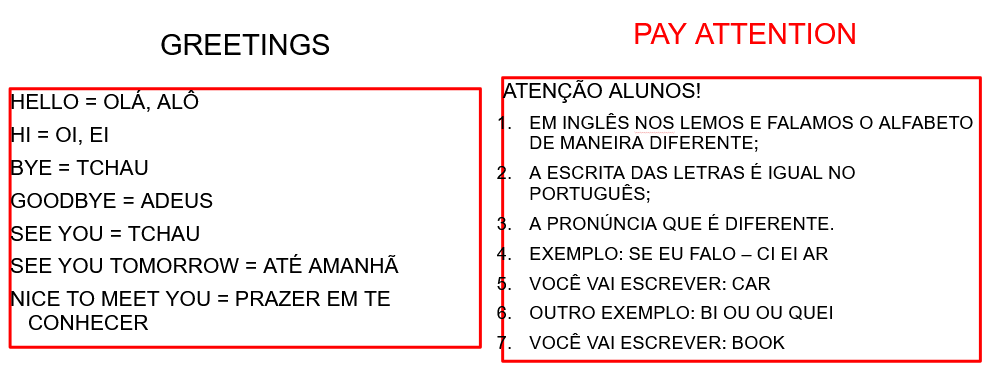
\includegraphics[width=\textwidth]{Fig1.png}
 \caption{Example of two slides made and used by the teacher to teach greetings and the alphabet.}
 \label{fig01}
 \source{Files made available by the interviewed teacher.}
\end{minipage}
\end{figure}

In terms of content, a relevant portion of the texts displayed in the slides are in Portuguese, whereas the English language is restricted to examples and exercises. These bear resemblance to the main characteristics of the grammar-translation method \cite{brown2006principles, harmer2007practice, richards2014approaches} of teaching, as seen:

\begin{quote}
1. Classes are taught in the mother tongue, with little active use of the target language.
2. Much vocabulary is taught in the form of lists of isolated words.
3. Long elaborate explanations of the intricacies of grammar are given.
4. Grammar provides the rules for putting words together, and instruction often focuses on the form and inflection of words. […] 7. Often the only drills are exercises in translating disconnected sentences from the target language into the mother tongue. […] \apud[p. 3]{prator}[p. 18-19]{brown2000douglas}

\end{quote}

With little to no attention to the learners’ needs or interests, this method has been known, according to \textcite[p. 7]{richards2014approaches}, to often bring “frustration for students” and to offer a “tedious experience of memorizing endless lists of unusable grammar rules and vocabulary”. Not only that, since the grammar-translation method focuses mostly on the grammar points of the target language, it is also said that “students have little motivation to go beyond grammar analogies, translations and rote exercises" \cite[p. 19]{brown2000douglas} when faced with this alternative in language classes. All these aspects, in our understanding, ultimately, seem to relate to the problem of motivation and engagement in the classroom first brought up by the teacher in our interview.


\subsection{Data collection and analysis: class observation}

It was with the intent of testifying the lack of motivation and engagement of the students, first described by the interviewed teacher, and investigating its main causes that we decided to observe one of the English online classes taught by Lavinia through Google Meet platform. This specific class happened on June 24th and had an average of 35 students online throughout the session, lasting only 36 minutes – 14 minutes less than the average allotted time for school classes in Brazil. We, then, decided to manually count students’ participation (here understood as any type of manifestation related to the class itself) both through audio and the chat area available on Google Meet’s interface (\Cref{tab1}).

\begin{table}[h!]
\centering
\begin{threeparttable}
\caption{Students’ engagement data on June 24th.}
\label{tab1}
\begin{tabular}{lr}
\toprule
Total number of students registered & 117         \\
\midrule
Maximum number of students online & 44 (100\%)           \\
Average number of students online & 35 (79\%)            \\
Students who engaged at least once with the activities & 11(25\%)  \\
Students who engaged more than once with the activities & 3 (27\%) \\
\bottomrule
\end{tabular}
\source{Made by the author.}
\end{threeparttable}
\end{table}

Matching our statements from the pedagogical material analysis, this class also presented a set of characteristics usually related to the grammar-translation method of teaching \cite{brown2000douglas, harmer2007practice, richards2014approaches}. The mother tongue, for example, was used in every single interaction with students. Vocabulary, taught out of context of usage and in form of lists of words, was expected to have been memorized. Most of the activities were presented first as a translation exercise, and, as seen in \Cref{fig02}, then as a fill-in-the-blanks type of activity, with little to no connection to the students’ personal interests and social or cultural contexts.

\begin{figure}[htbp]
\centering
\begin{minipage}{.8\textwidth}
 
\includegraphics[width=\textwidth]{Fig2.png}
 \caption{Sample of activities used in a review class on June 24th}
 \label{fig02}
 \source{Files screen-captured during the observed class on June 24th. Original file available at All Things Grammar \url{https://www.allthingsgrammar.com/adjectives-and-adverbs.html} Last access: 04 mai. 2023.}
\end{minipage}
\end{figure}

Another relevant comment that should be made about this specific class is that the teacher rarely used students’ names when referring to them. From the observer’s perspective, it seemed to be difficult for Lavinia to recognize her students’ voices through the audio interactions. Not only that, it was not uncommon to hear her complaining in a low voice through the microphone whenever a student made a wrong guess. Both aspects, as it is possible to infer from \Cref{tab1}, seemed to discourage students from taking risks and, consequently, from further engaging in new activities. Mistakes were never clarified as to why they would configure mistakes, leaving students clueless in regard to the reasons that their answers were not accepted. Finally, as \Cref{fig02} shows, the activities were not personalized to the students’ needs and interests, rather, all of them were downloaded from the internet and presented in a vertical layout – which impairs reading on small screens.


\subsection{Data collection and analysis: questionnaire}

As the next step of this research involved teaching in the specified context, we sought to understand the students’ personal interests and general involvement with game mechanics, in-class activities and digital media, as well as their own lives and routines outside the school field. In order to visualize the exact context in which the teaching practice would, at a later date, occur, we prepared an online questionnaire that was posted on July 13th through their Google Classroom homepage. Ranging from open-ended questions that allowed students to freely write about themselves, to close-ended questions that focused on understanding their favorite songs, TV programs, games and classroom activities, this step allowed us to collect 31 different answers that provided relevant data for the proposal of our first lesson that was scheduled to happen on August 9th.

Through the open-ended questions, we were able to rank the students’ five favorite leisure activities, which included: a) browsing Instagram and TikTok (67,70\%); b) playing games both on computer and video game consoles (64,50\%); c) playing card or board games (45,20\%); d) chatting with friends and colleagues (45,20\%); and e) watching cartoons (41,90\%). Now, in regard to the students’ favorite classroom activities, most answers revealed that they enjoy: a) Activities with music (71\%); b) Movies, TV series and cartoons in English (67,7\%); c) Dialogue activities (58.1\%); and d) Educational Games (58,4\%). The least voted alternative was fill-in-the-blanks activities (19,4\%), which, surprisingly, is thoroughly used by their English teacher.

Finally, the last question was open-ended and invited students to share a bit about themselves and their personal interests. Some of them chose to use the free space to highlight their interest both in English, as a subject, and in classes with games and opportunities for interaction. Apart from one student, who manifested her interest in learning English as a means of watching movies and series in their original language without subtitles, no one mentioned reasons as to why they were learning English. That, of course, is understandable, as English is a mandatory class to be taken at regular schools. One student stated that she enjoyed classes the most when the teacher would “play a bit with students” and when “everyone could have a nice chat”. Not only that, but at least three different students pointed out that they enjoyed practicing English outside the classroom using either smartphone applications or YouTube videos. These bits of information point out that, at least for these participants, learning English could be either enjoyable, interesting or relevant enough for them to use their free time to learn it outside classroom time.


\subsection{Data collection and analysis: lesson plan and class teaching}

Through the review of the literature already presented and using all the data collected up to this point, we decided that placing the students’ responses to the questionnaire at the center of the lesson design would be the best approach as to evaluate if elements such as gamification and learner-centered instructions would have a decisive impact on class participation. With that in mind, the first class designed inherited a set of elements from game design logics \cite{deterding2011game}, such as team division, scoreboards and leaderboards, turns, a variety of game styles and a playcentric design that focused on the cooperative aspect \cite{felder1996navigating} that is natural to student-centered instructions. The whole class was prepared with reference to mass-media entertainment products previously referenced in the questionnaire (see \Cref{fig04} and \Cref{fig05}), bringing forth characters, cartoon animations, comics and pieces of music that were suggested by the students themselves. Not only that, resources and features from popular smartphone applications such as TikTok, for example, were also included in some of the activities.

\begin{figure}[htbp]
\centering
\begin{minipage}{.8\textwidth}
 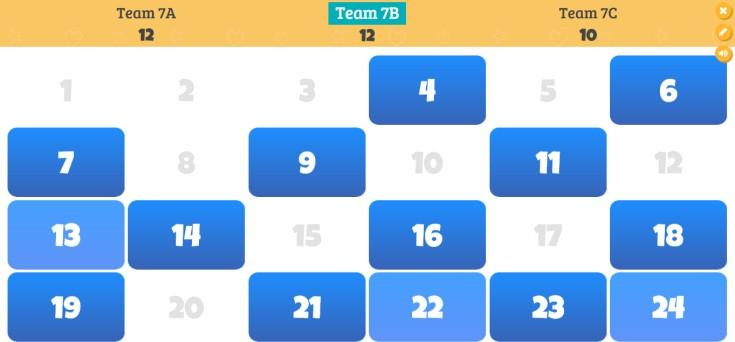
\includegraphics[width=\textwidth]{Fig3.jpg}
 \caption{Baamboozle board used for teaching}
 \label{fig03}
 \source{Made by the author.}
\end{minipage}
\end{figure}

The class was then planned with the intent of reviewing the same concepts that were previously taught, such as adjectives, means of transportation and the To Be verb in present tense. The main platform used to first develop the class was Baamboozle (\Cref{fig03}), a \emph{freemium} tool for creating and playing online educational games that allows users to customize questions, images and possible answers for each card, creating a simulation of a board for turn-based games.

Each card would present the team with an activity, that ranged from riddles with vocabulary, character description prompts, dialogue challenges, music activities and speaking tasks that prompted students to talk about their interests and interact with either cartoons, videos from TikTok or with the teacher.

\begin{figure}[h!]
\centering
\begin{minipage}{.8\textwidth}
 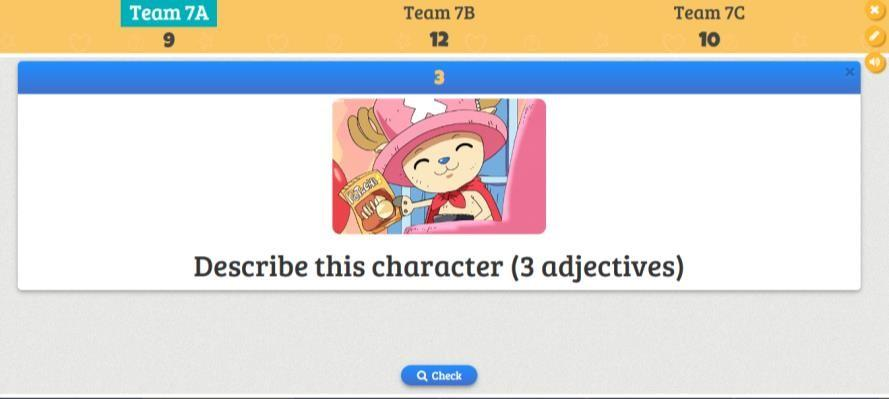
\includegraphics[width=\textwidth]{Fig4.jpg}
 \caption{Sample of a card used in lesson}
 \label{fig04}
 \source{Made by the author using Baamboozle.}
\end{minipage}
\end{figure}

Video and music activities were also presented through the Google Slides platform, using the Baamboozle board as a hub for all possible review activities in this class. In both music and video tasks, students were able to select their theme of interest through a manually made menu that simulated the concept of a playlist (made, again, from the suggestions first presented in the questionnaire).

\begin{figure}[h!]
\centering
\begin{minipage}{.8\textwidth}
 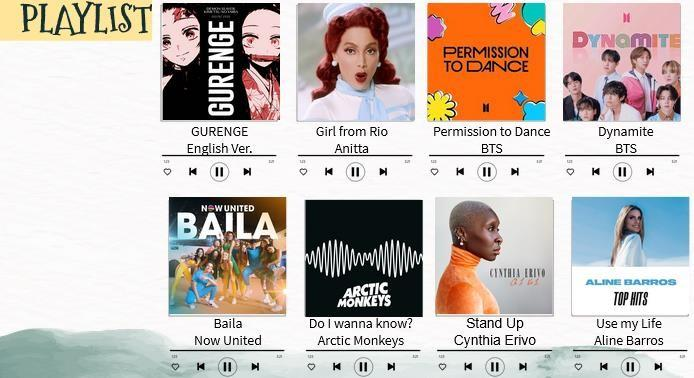
\includegraphics[width=\textwidth]{Fig5.jpg}
 \caption{Sample of the playlist presented for music activities}
 \label{fig05}
 \source{Made by the author.}
\end{minipage}
\end{figure}

Each song had a different kind of activity attached to it, ranging from tasks such as lyric matching, lyric reorganizing, spotting the mistakes, guessing the missing words, rhyme finding etc. This was made, first and foremost, with the intent of giving students a certain sense of control over the content being taught \cite{harmer2007practice, ryan2009promoting}, allowing them to navigate over themes, tasks and products that they would mostly relate to. These types of games and opportunities for active learning, as stated by \textcite{ryan2009promoting}, are intrinsically motivated activities that should prove useful for our action-research, as they might boost engagement in classroom because of the overall sense of competence and autonomy that comes from solving these tasks, getting points for your own team and interacting with contents personally chosen by the students themselves.

A second class was planned following the same principles of SCI and gamification, however, this time, the main objective was to present the simple past tense of the “to be” verb using a more collaborative approach. Students were first introduced to a set of Instagram posts and YouTube comments that displayed the use of the simple past tense of “to be”. Then, using the structure they had just seen through the comments, we invited students to “duet” – a trend among users of TikTok in which you simulate a dialogue with another user – first, with me, then, with their colleagues, using dialogues sample from cartoons they had suggested after the EFL class last taught on August 9th. Following another game-design element, each duet was placed into four different levels that had ascending difficulty, forming a progressive learning curve. So, by the time students reached the fifth level – the last one – they were already used to the manipulation of the verb to be in the past tense and were able to complete it with ease – even if the activities themselves were harder and trickier than the ones from the first level presented in \Cref{fig06}. Some activities missed not only the verb but also the pronouns, adjectives and so on, requiring that students completed the conversation with either their own info or with the lore from the cartoon they had chosen.

\begin{figure}[h!]
\centering
\begin{minipage}{.8\textwidth}
 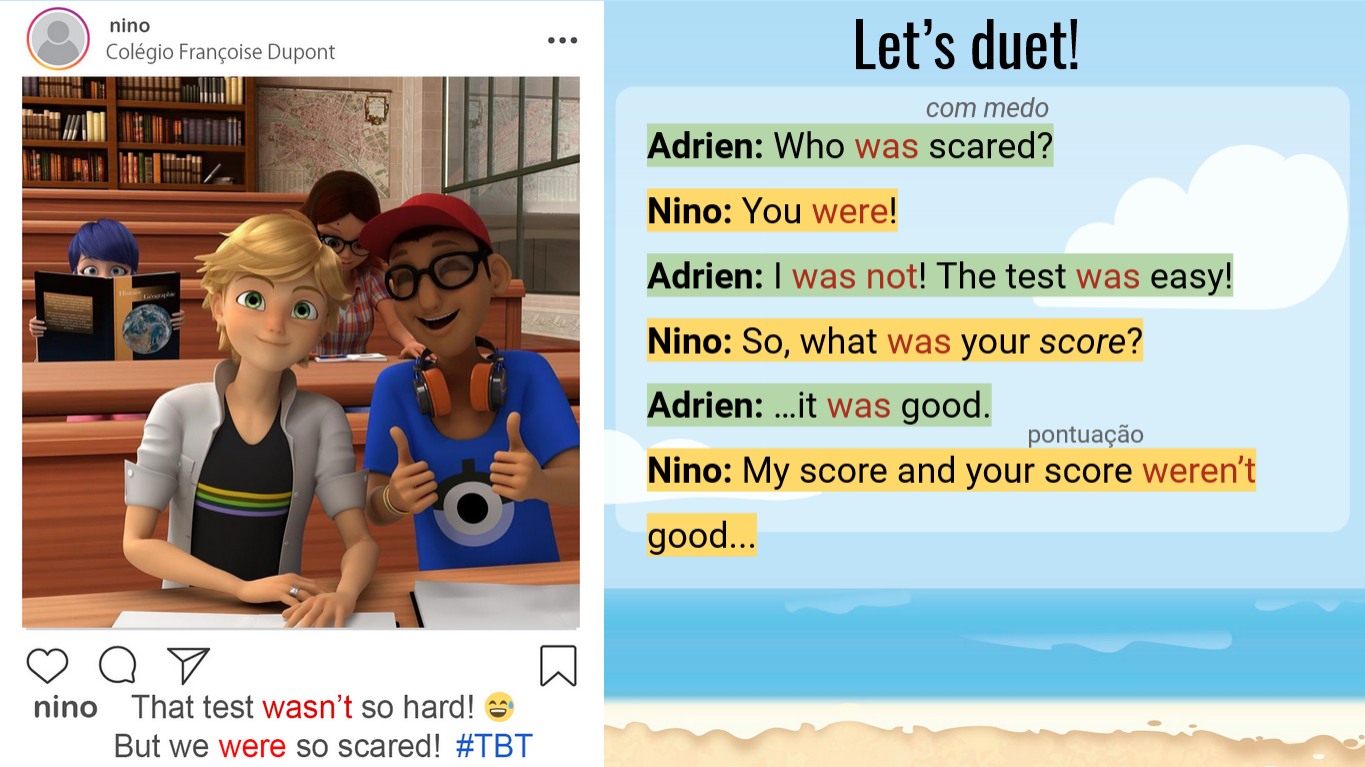
\includegraphics[width=\textwidth]{Fig6.png}
 \caption{Sample of the dialogue performed by students}
 \label{fig06}
 \source{Slides made by the author.}
\end{minipage}
\end{figure}


\section{Results}

After conducting the two planned classes, we were able to replicate the same method used to measure classroom participation in Lavinia’s classes on our own. The results are displayed in the \Cref{tab2}.

\begin{table}[h!]
\centering
\begin{threeparttable}
\caption{Students’ engagement data comparison}
\label{tab2}
\begin{tabular}{p{6cm}lll}
\toprule
Lesson date: & June 24th & August 9th & August 16th \\
\midrule
Teacher responsible for the class & Lavínia & Researcher & Researcher \\
Class’s length  & 36 minutes  & 47 minutes & 49 minutes \\
Total number of students registered & 117 & 117 & 117                  \\
Maximum number of students online & 44 (100\%) & 29 (100\%)           & 32 (100\%) \\
Average number of students online & 35 (79\%) & 27 (93\%) & 30 (94\%)            \\
Students who engaged at least once & 11 (25\%) & 21 (72\%)            & 19 (59\%) \\
Students who engaged more than once & 3 (27\%) & 20 (95\%) & 19 (100\% ) \\
\bottomrule
\end{tabular}
\source{Made by the author.}
\end{threeparttable}
\end{table}

First, comparing the total number of students enrolled in this class (117 students) and the average attendance per class (44, 29 and 32), it’s possible to note that, as Lavínia had first mentioned, the number of students coming to classes is, indeed, low. 

For June 24th, for example, we had only 37.6\% (44) students coming to classes, and that low percentage is still noticeable within both classes taught by us. On August 9th we had only 24.7\% (29) of the total students in class, and on August 16th we had only 25.6\% (30) of students attending the online class. Between June 24th and August 9th students in this specific school had a test week, and, according to the teacher, this decrease in attendance (from 44 to 29 students in class) was expected, as they tend to miss classes immediately after their tests as it’s often believed that these classes won’t bring new relevant content that would impact on students’ performance in the following test. Of course, this short period of time wasn’t enough for us to evaluate if the newly planned and conducted classes would have a direct impact on attendance, per se. It would be interesting to further evaluate how the sudden change in the teaching approach used might affect student’s retention in the classroom in the long term.

Now, comparing both Lavinia’s (June 24th) class and our first class (August 9th), it is possible to notice that, even though our class had significantly fewer online students (13\%), these very students that were present were much more engaged with the proposed activities when compared to the class taught on June 24th. While Lavinia’s class had only 31\% of the students’ engagement (considering the average number of online users), both of our classes taught in August had a percentage of interaction of 78\% and 63\% respectively when considering the average number of students online. Above all, we should point out that 95\% of the students who had engaged in any of the activities proposed in August 9th’s class, willingly reengaged either through audio or chat messages. That number is even higher in August 16th’s class, where all students (100\%) who had previously engaged decided to repeat their participation. However, in June that number amounts to only 27\% of students who had previously participated.

We were also able to observe a second class taught by Lavinia that happened on August 30th, three days after our last taught class and after having discussed with the teacher the results observed so far. Again, no interaction seemed to happen between the students and the content being presented. The teacher maintained the grammar-translation approach previously appointed while teaching the simple past tense of regular verbs in English – which means that out-of-context lists of vocabulary were used whilst giving special emphasis to grammatical rules through repetition and memorization of content. Noticing that no students were responding to her class, she decided, then, to carry out a spelling activity in the chat area of the Google Meet app and prompted students to take part as she would be “carefully observing who was and who was not participating”. Since this kind of interaction was prompted by a thin-veiled threat, we decided not to compute it in the chart above, as it was not an organic-kind of engagement as were the ones registered since the first class. For this class, just like the one from August 16th, we had an average number of 30 students online, with no spontaneous participation stemming from the students. 16 (53\% of the average number online) students were name-prompted by the teacher to answer her questions, and none of them (0\% of these 16 students) willingly re-engaged with the activity. We understand that the tension of being “carefully observed”, as said by the teacher, and the type of language used in order to elicit their participation (sentences such as “we studied that already, why can’t you answer it correctly?” or “your classmates know the answer, why are you the only one who doesn't know it?" were often used in a derogatory way during the activity) sparked a sense of anxiety in the students and waned their willingness to voluntarily interact with the subject. Throughout both lessons we taught we did notice that students were, actually, interested in participating and voicing their impressions of the subject, but in order to do that, they needed to feel not only safe when doing so but also welcomed even when committing mistakes.

While using game-design elements surely helped in making the class more enjoyable and novel to students, our understanding is that bringing references to content chosen by the participants themselves, valuing their voices in the making of the lesson, offering positive and relevant feedback throughout the teaching process and offering a certain degree of autonomy contributed to these students being increasingly willing to participate in class activities. Game elements, as pointed out by \textcite{koivisto2019rise}, are not always the perfect solution for an unmotivated classroom. The short nature of the experiment here described did not allow for a long-term evaluation of the strategy of gamifying the lessons, but it is not hard to predict that the element of novelty would soon fade, especially if the students had not manifested previous interest or experience in games. If taken isolated, the employment of new, adjusted game strategies would have been needed in order to keep students continuously challenged by the class’ format. Moreover, the instantaneous gratification brought forth by the positive feedback immediate to students’ participation could create an environment in which engaging with the content is always conditioned to an unstable external element. In our case, this element is firmly attached to the teacher’s response to participation in class rather than to elements that students would be able to maintain under different conditions. 

While the desire for recognition also plays its part within the logic of motivation and within students’ interest in partaking in the proposed activities, conditioning one’s posture towards the learning process only to the reaction of the other is a frail bet that is not able to uphold motivation as a whole. One clear example is how that dependence turned against students when they did not find the same positive response to their engagement as the ones offered during classes taught on August 9th and 16th. Thus, while the gamified approach did bring positive results to this research, it was not, and it should not be taken as, the sole element responsible for an engaging class. Not only that, \textcite{aguilos2022perceived} discuss how this instant gratification may appeal positively to highly competitive students, but, what about students with different profiles? The competitive aspect that often comes with gamified experiences, and the pressure or demand for recognition through the positive feedback, could very well wear out students that do not find pleasure in this kind of setting. Gamification, as any other strategy centered in the student, should always be considered while having their personalities, identities, contexts and experiences as the departing point. Finally,  observing and developing strategies to address the imbalance of power that might also manifest or emerge from this kind of online gamified experience is also fundamental to a class that aims to promote an enjoyable and collaborative environment at its core, as the access and representation in digital games is still deeply marked by aspects of both gender and race \cite{leonard2006not,kelly2023you}.

 Besides the positive feedback, referencing students by name made them more eager to engage with the class. During both classes, we focused on ensuring that the learning environment was inviting – meaning that we reinforced the validity of every type of participation in the resolution of activities. Bringing out a human approach to interacting with students allowed them to feel at ease even when making incorrect guesses about the tasks presented. The mistakes were treated with utmost care (students who made wrong guesses, for example, were never called out, instead, we would go back some slides and re-explain the content to help them notice their own mistakes), and students who had first encountered them were still willing to participate and to keep on guessing and changing their answers – mostly, for the sake of participating.

Affect had a huge impact on these specific students. Finding out that they were able to contribute to the classes’ progress and that they could, and should, speak up, allowed them to take more risks and to interact with the content in a way that seemed novel. As a result, at the end of each class, we were able to observe and register students’ impressions, which were not prompted by us at any given time, on the whole process, and the overall response was highly positive. Some students asked when our next class would take place so that they would not miss it. Other students thanked for the class, saying that it was fun and, in their own words, “perfect”.

Providing an environment that allows students to engage without the fear of being ostracized because of their “mistakes” allows them to establish positive affective connections between the content and the learning process. In addition, showing interest in cultural products that they also value seemed to evoke a sense of belonging in the classroom, which, naturally, has a huge impact on both motivation and on their particular notion of identity. In this scenario, the concept of investment helps us move from an approach that conceptualizes students as binary beings with variables that exist independently (motivated or unmotivated? Competitive or noncompetitive? Introverted or Extroverted? “Good” student or “bad” student?) towards an approach that considers people as beings with multiple identities that are constantly being “negotiated through language and social interaction” \cite[p. 3]{darvin2023investment}. Motivation cannot, and should not, be seen as an independent variable that is possible to tackle through a void. That is why investment brings a counterpoint to this concept, as it highlights the constant struggle that students face when renegotiating their own identities even while learning a new language. With SCI it is possible to elevate the logic of student’s identity as a central point in the teaching process but only through an informed approach that acknowledges the tension that arises from the power imbalance in that specific context.

Following this logic, the success observed in this experiment can be attributed more to the possibility of students manifesting their interests and seeing those interests being validated inside the classroom, than to the fact that the content was introduced through game mechanics. The nature of both the language used and the social interactions observed during the two classes that we taught was fundamentally different from those observed in the other classes. That aspect, per se, changes the context of learning and directly impacts on the way these students negotiate their own identities through discourse. Investment, here, emerges as a variable that, even if not explicitly considered in the development of our research, sheds light on aspects that were, if not more relevant, at least, more immediate to be approached in that specific classroom.

Before concluding, there is one last aspect that must be addressed: no amount of creativity in class is enough to remediate the perception of being trapped under dire working conditions. Lavinia’s crystalized sense of hopelessness as a teacher in Brazil is not new \cite{barcelos2018emotions}, and it does affect the way she addresses students as well as the types of classes she is able to plan and conduct. Systemic problems, such as the undervaluation of the teacher’s career, for example, undermine classroom engagement when those involved with it are not able to interact with the learning environment without feeling constrained by the amassing difficulties that appear on their way: lack of proper materials to watch and participate in class, lack of training, lack of support from the school, lack of a positive sense of identity within the learning context etc. From within those problems, no gamification and SCI are enough to provide a solution to the perceived lack of motivation. Even with a positive result, it is important to remember that the experiment conducted here is an exception to the routine of the classroom, and that structural problems should always be taken into consideration as crucial factors to the motivation of both students and teachers alike.

\section{Acknowledgement}

I would like to express my deepest gratitude to Professor Leina Cláudia Viana Jucá (UFMG), my research supervisor, for her patient guidance, enthusiastic encouragement and useful critiques, without which I would never have finished this research work.




\printbibliography\label{sec-bib}
% if the text is not in Portuguese, it might be necessary to use the code below instead to print the correct ABNT abbreviations [s.n.], [s.l.]
%\begin{portuguese}
%\printbibliography[title={Bibliography}]
%\end{portuguese}


\end{document}

